\subsection{Roundoff By Area}
The simplest way to round off is to take every small unit (we will 
use counties in this example) and find the larger unit (districts) 
which contains the largest portion of its area. For example, 
consider two districts which partition a square region split 
up into four counties:
\begin{center}
  \resizebox{0.2\textwidth}{!}{
  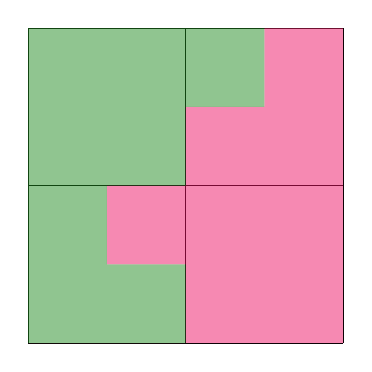
\begin{tikzpicture}
    \draw[\thicc, xstep = 2, ystep = 2] (0,0) grid (4,4);
    %\draw plot[smooth, tension = 0.5] coordinates {(0,0) (0.5,1) (1,2) (2,2) (3,3.5) (4,4)};
    \fill [\thicc, opacity = .5, WildStrawberry] (0,0) -- 
    (2,0) -- (2,1) -- (1,1) -- (1,2) -- (2,2) -- (2,3) -- (3,3) -- 
    (3,4) -- (4,4) -- (4,0) -- (0,0);
    \fill [\thicc, opacity = .5, ForestGreen] (0,0) -- (2,0) -- (2,1) -- 
    (2,0) -- (2,1) -- (1,1) -- (1,2) -- (2,2) -- (2,3) -- (3,3) -- 
    (3,4) -- (4,4) -- (0,4) -- (0,0);
    % \node (C1) at (0,0) {};
    % \node (C2) at (0.5,0.1) {};
    % \node (C3) at (0.6,0.3) {};
    % \node (C4) at (0.5,0.6) {};
    % \node (C5) at (-0.1,0.7) {};
    % \node (C6) at (-0.3,0.65) {};
    % \node (C7) at (-0.4,0.5) {};
    % \node (C8) at (-0.4,0.1) {};
    %\draw plot [smooth, tension = 0.5] coordinates 
    %{(0,0) (0.5,0.1) (0.6,0.3)
    %(0.5,0.6) (-0.1,0.7) (-0.3,0.65)
    %(-0.4,0.5) (-0.4,0.1) (0,0)};
    %\addplot [smooth] nodes {(0,0) C2};
    %\draw plot [smooth] C1 -- C2 -- C3 -- C4 -- C5 -- C6 -- C7 -- C8;
  \end{tikzpicture}
  }
\end{center}
Under the area method of roundoff, the district association of the 
counties becomes:
\begin{center}
  \resizebox{0.2\textwidth}{!}{
  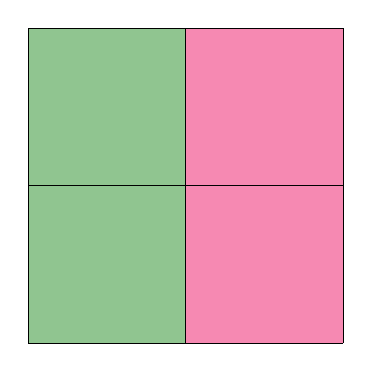
\begin{tikzpicture}
    \fill [opacity = .5, WildStrawberry] (2,0) rectangle (4,4);
    \fill [opacity = .5, ForestGreen] (0,0) rectangle (2,4);
    \draw[\thicc, xstep = 2, ystep = 2] (0,0) grid (4,4);
  \end{tikzpicture}
  }
\end{center}
Note that there is a minute chance that two districts may contain 
an equal amount of a county's area, and no other districts contain as 
much area. In this case, the algorithm will just toss a coin. However, 
in real data, this is extremely rare.
\subsection{Roundoff by Population}
In this method of roundoff, we assume that both the districts 
and the counties are composed of the same base building blocks, 
with populations attached. In this case, we 
associate a county to the district containing the largest portion 
of its population. For example, in the above, if the counties 
were further subdivided into squares with populations:
\begin{center}
  \resizebox{0.2\textwidth}{!}{
  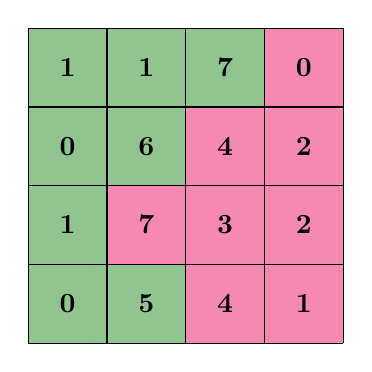
\begin{tikzpicture}
    \fill [\thicc, opacity = .5, WildStrawberry] (0,0) -- 
    (2,0) -- (2,1) -- (1,1) -- (1,2) -- (2,2) -- (2,3) -- (3,3) -- 
    (3,4) -- (4,4) -- (4,0) -- (0,0);
    \fill [\thicc, opacity = .5, ForestGreen] (0,0) -- (2,0) -- (2,1) -- 
    (2,0) -- (2,1) -- (1,1) -- (1,2) -- (2,2) -- (2,3) -- (3,3) -- 
    (3,4) -- (4,4) -- (0,4) -- (0,0);
    \draw[\thicc, xstep = 2, ystep = 2] (0,0) grid (4,4);
    \draw (0,0) grid (4,4);
    \node at (0.5,0.5) {\bf 0};
    \node at (1.5,0.5) {\bf 5};
    \node at (0.5,1.5) {\bf 1};
    \node at (1.5,1.5) {\bf 7};


    \node at (2.5,0.5) {\bf 4};
    \node at (3.5,0.5) {\bf 1};
    \node at (2.5,1.5) {\bf 3};
    \node at (3.5,1.5) {\bf 2};


    \node at (0.5,2.5) {\bf 0};
    \node at (0.5,3.5) {\bf 1};
    \node at (1.5,2.5) {\bf 6};
    \node at (1.5,3.5) {\bf 1};

    \node at (2.5,2.5) {\bf 4};
    \node at (2.5,3.5) {\bf 7};
    \node at (3.5,2.5) {\bf 2};
    \node at (3.5,3.5) {\bf 0};
  \end{tikzpicture}
  }
\end{center}
then the roundoff by population would look like:
\begin{center}
  \resizebox{0.2\textwidth}{!}{
  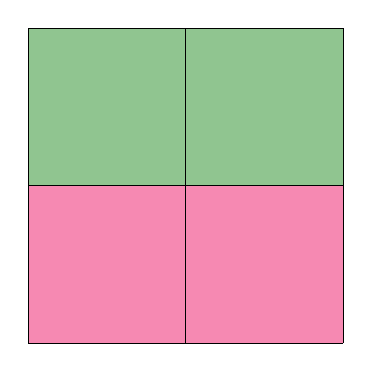
\begin{tikzpicture}
    \fill [opacity = .5, WildStrawberry] (0,0) rectangle (4,2);
    \fill [opacity = .5, ForestGreen] (0,2) rectangle (4,4);
    \draw[\thicc, xstep = 2, ystep = 2] (0,0) grid (4,4);
  \end{tikzpicture}
  }
\end{center}
